\documentclass[conference]{IEEEtran}

\newtheorem{definition}{Definition}
\usepackage{algorithm}
\usepackage{algpseudocode}
\usepackage{float}
\usepackage{moreverb}
\usepackage{subfigure}
\usepackage{graphicx}
\usepackage{url}

\usepackage{tikz}
%%%%% This is used to strike out text in latex %%%%%%%%
\usepackage[normalem]{ulem}
\newcommand\redsout{\bgroup\markoverwith{\textcolor{red}{\rule[0.5ex]{2pt}{0.4pt}}}\ULon}
%%%%%%%%%%%%%%%%%%%%%%%%%%%%%%%%%%%%%%%%%%%%%%%%%%%%%%%



\makeatletter
\@addtoreset{equation}{section}
\makeatother
\renewcommand{\theequation}{\arabic{section}.\arabic{equation}}
%=============================================================================
\newtheorem{theorem}{Theorem}    [section]
\newtheorem{remark}{Remark}   [section]
\newtheorem{corollary}{Corollary}  [section]
\newtheorem{lemma}{Lemma}    [section]
\newtheorem{conjecture}{Conjecture} [section]
\newtheorem{example}{Example}    [section]


\newcommand\BibTeX{{\rmfamily B\kern-.05em \textsc{i\kern-.025em b}\kern-.08em
T\kern-.1667em\lower.7ex\hbox{E}\kern-.125emX}}

 
% Figures path in the folder - Added Fkandah
%%%%%%%%%%%%%%%%%%%%%%%%%%
\graphicspath{{./Figures/}} % Define the figures path %
%%%%%%%%%%%%%%%%%%%%%%%%%%


%%%%%%  Added by F.Kandah - April 27, 2018  %%%%%%%%%%%%
                                                    %%
\usepackage[english]{babel}                         %%
\usepackage[autostyle,english=american]{csquotes}   %%
\MakeOuterQuote{"}                                  %%
%%%%%%%%%%%%%%%%%%%%%%%%%%%%%%%%%%%%%%%%%%%%%%%%%%%%%%

% correct bad hyphenation here
\hyphenation{op-tical net-works semi-conduc-tor}

%%%%%%%%%%%%%%%%%%%%%%%%%%%%%%%%%%%%%%%%%%%%%%%%%%
%%%%%%%%%%%%%%%%%%%%%%%%%%%%%%%%%%%%%%%%%%%%%%%%%%
%%%%%%%%%%%%%%%%%%%%%%%%%%%%%%%%%%%%%%%%%%%%%%%%%%

\begin{document}

%%%% Your paper title goes here . . . . .
\title{Forecasting Fatality Outcomes for COVID-19 in the United States of America}


% author names and affiliations
\author{Paul Aidan Smith \\
\IEEEauthorblockA{\textit{College of Engineering and Computer Science} \\
\textit{University of Tennessee at Chattanooga}\\
Chattanooga, Tennessee \\
4/18/2020}
}

\maketitle

\begin{abstract}
In December 2019, a novel coronavirus strain emerged in Wuhan, China.  In the following months, the spread of the pandemic has grinded the world to a halt.  Worldwide case and fatality data has been well documented for the United States of America, leading to many data scientists and epidemiologists creating models to simulate and forecast outcomes for this virus.  These models have been a bit of a mixed-bag, with some being very good and others poor. This paper sets out to analyze the spread of COVID-19 in the United States, focusing on forecasting fatality rates.  Additionally, it aims to compare and contrast this modeling with some of the largely cited models currently being used. This model attempts to adapt to different scenarios in order to analyze different outcomes from varying levels of fatality rates, population of cases, and time delay between infection and death.

While the United States has observed social distancing and other minimization efforts, the healthcare demand is likely going to far exceed the supply due to the COVID-19 pandemic.  This systematic risk has been seen firsthand in countries struck earlier in the lifecycle of the spread, such as Italy and Spain.  As it spreads throughout the United States, it is very critical to get the best possible forecasts in order to properly model the fatality impacts of COVID-19. 

\end{abstract}


\section{Introduction}
\label{Intro}

In early December 2019, the novel coronavirus (severe acute respiratory syndrome [SARS]- COV-2, also known as COVID-19) was first identified from patients with severe pnemonia-like symptoms \cite{long} .  In the next several months, this Coronavirus spread globally and turned into a worldwide pandemic.  The spread and impact of this novel virus has been a major problem globally, but the United States has been greatly effected.  This paper aims to address and analyze the impact of COVID-19 in the United States, as well as discuss several of the many models that attempt to forecast fatality impacts.  

    COVID-19 is not only causing mortality, but also comes with large systemic risk to the healthcare system.  There has been many comparisons to the flu by the media, however COVID-19 brings significantly more risk due to the unpredictability and lack of a vaccine.  As we have seen in Italy and many other countries, healthcare systems have been overrun with COVID-19 cases.  This results in triage measures due to lack of hospital beds, ventilators, and available staff, which greatly inflates the fatality rate and overall fatalities.  Accurately modeling this risk is paramount in order to accurately forecast the demand for these Intensive Care health resources in order to minimize the death toll of this virus.
    
    Learning more about this disease and its attributes is essential for any modeling to be done.  In epidemiology, R\textsubscript{0} is a mathematical term that indicates how contagious an infectious disease is.  R\textsubscript{0} tells you the average number of people who will catch a disease from one contagious person.  COVID-19 has an estimated R\textsubscript{0} of 2.4 \cite{who}.  Additionally, variables such as the amount of confirmed cases, and the time delay between infection and death are critical to forecasting the impact on the health system.  Unfortunately due to lack of mass testing, the amount of confirmed cases is merely a function of the amount of tests being performed.  Thus, to get a good estimate, the total case population must be calculated to get a more accurate number.
    
    There have been several cited models touted by President Trump and the Coronavirus Task Force.  The one most widely used is from the Institute for Health Metrics and Evaluation (IHME) \cite{imhe}.  However, this model seems to considerably under-predict projected fatalities.  Similarly, the CovidActNow model seems to over-project fatalities by making poor assumptions on reproductive number of infections\cite{covidactnow}.  The Los Alamos group model is the best one out there that is close to the actual numbers \cite{losalamos}.  However, all models are likely flawed as this is a very tough problem to solve and model. 

%\vskip .01in
%\includegraphics[scale=.125]{Figures/Net_Illustration (1).jpg}  
%\caption{ A wireless sensor network}

\section{Methods}
\label{Methods}

Attempting to accurately forecast the fatality impact of COVID-19 requires understanding the underlying variables present in the disease.  These include the R\typesubscript{0}, the fatality rate, the amount of active cases, hospital utilization percentage, and the time delay between contracting the disease and death.  Using estimates for the fatality rate and time delay between contraction and demise, the amount of active cases can be interpolated.  As previously mentioned, due to lack of mass testing in the United States, relying on the actual data for total cases is unwise.  This total case data is largely just a function of total tests, rather than a true measure of the total active cases.  All daily case data was retrieved from Johns Hopkins University and Medicine Coronavirus Resource Center \cite{JHU}. While the "confirmed cases" data can be suspect, the death data is accurate and as immune to undertesting as it can be.  The only caveat being that fatalities that are not reported due to not going to the hospital are not captured.  The United States is currently at 31,456 deaths \cite{JHU}.  From this data, hypotheses can be constructed about the progression of the illness.

Using the Johns Hopkins time series of US deaths, we can easily reconstruct how many Americans had the coronavirus three weeks prior.  A case fatality rate of 1.54 percent is used, which comes from cases on cruise ships where 100 percent of passengers were tested \cite{ships}.  This level is obviously an estimate that leads to the largest source of model uncertainty, so the Shiny application developed allows for customizable user input to adjust to more certain rates. In the effect of overwhelmed healthcare systems and intensive care resources, the fatality rate would likely rise much higher.  Three weeks was defined as the time delay between contracting the infection and death.  This is consistent with the median 6 days to symptoms and 13 days to death cited from the Center of Disease Control \cite{cdc}.

A lower fatality rate is a bit of a double-edged sword in this analysis.  If the true fatality rate was 0.1 percent, then this analysis would show 10 times as many calculated infected people.  This model is simplistic and does not account for people being cured and developing antibody immunity, the effects of social distancing and lockdown, and innacuracies in fatality rate reporting.  Nonetheless, the model shows an estimated 385,700 new daily cases for March 28, 2020, versus the actual report of 19,733 \cite{JHU}.  This is a dramatic divergence, but relatively consistent with reports stating that the actual cases represented just 6 percent of infections on average across 40 national governments at the end of March \cite{reason}.  Applying that 6 percent would estimate the total cases on March 28 to be 328,883.

To model the daily deaths, the data was fit to a 2nd order polynomial regression model, adjusted to per capita numbers.  Due to lack of decreasing daily fatalities in the United States, it was difficult to fit a model that would ever come back down to 0.  Many of the cited models did a far more complicated analysis with SIR differential equations that give more scientific predictions.  Using several countries per capita daily fatality curves, I applied the model to the United States current shape. China data was not used in this analysis, due to questions about its accuracy and sharp decline in fatalities. 

\section{Results}
\label{Results}

Forecasting this data was a definite challenge, and many of the more advanced statistical modeling methods would not adequately predict future data.  An initial approach to my time series forecasting efforts was using an Auto-Regressive Integrated Moving Average (ARIMA) model, but due to not having the decreasing trend present in the data, it performed very poorly.  After trying decomposition forecasting and receiving similar results, I resorted back to a basic polynomial regression.  I believe if I had more future data in the time series, those would have been better performing models.  Figure \ref{modelACC} illustrates the results given a 1 percent fatality rate. 



\begin{figure}[ht]
\centerline{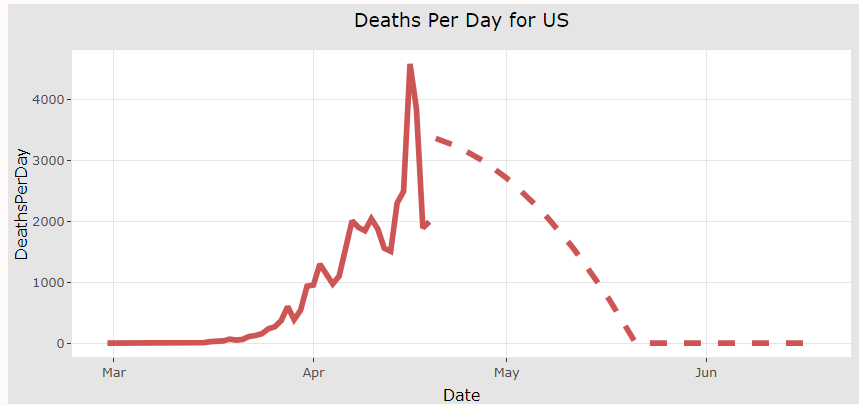
\includegraphics[scale=0.4]{Figures/Capture.PNG}}
\caption{Forecasting US Deaths Per Day}
\label{modelACC}
\end{figure}




While this quadratic rate of change is very simplistic and does not capture the full picture, it still gives an estimate of a hopeful decrease in daily fatalities.  The model predicts a drop to 0 daily deaths by early June.  This is likely not a realistic picture due to the plateauing nature observed in Italy and Spain. COVID-19 is an exponentially growing disease, so small differences in assumptions can make drastic effects on forecasts, and the data is not complete to illustrate the full picture.  Capturing R\typesubscript{0} over time as isolation and stay-at-home orders run their course is not an easy task.  

Another caveat of forecasting the fatality impact on the United States is the New York City metropolitan area's presence in the data.  This area was struck the hardest and the fastest with this pandemic, likely due to a massive and tightly congested population that relies so much on mass transit.  Many reports seem to suggest a decline in R\typesubscript{0} under 1, so cases are shrinking instead of growing.  While New York seems to be on the backside of this pandemic, many other regions are likely to increase in case load over the next several weeks, and the data is not convincing that the peak has been reached as a country.  This all depends on how open the public stays, and how effective social distancing can be in the United States compared to other countries with stricter guidelines. 


\section{Discussion}
\graphicspath{{Figures/}{../Figures/}}
\label{Discussion}
 As mentioned previously, there are many cited models touted by the press and scientific community.  The most popular one seems to be the Institute for Health Metrics and Evaluation (IHME) model \cite{imhe}.  This model has been considerably under-predicting projected death counts over the iterations of the model.  There are several assumptions at play that make this model questionable.  First, they assume a symmetric Gaussian-like curve for daily deaths and therefore a sigmoid-like curve for cumulative deaths.  There are epidemiological models that support this, but it remains to be seen if this will apply to different countries following different containment measures. Going back to smallpox outbreaks of the 1840's, William Farr showed that epidemics rise and fall in roughly a bell-shaped curve \cite{farr}.  Additionally, Farr stated topically that "The death rate is a fact; anything beyond this is an inference".  
 
 Assuming a Gaussian-like curve, we should expect to see shapes shown in Figure \ref{m3} when analyzing infections and deaths.

 \begin{figure}[H]
\centerline{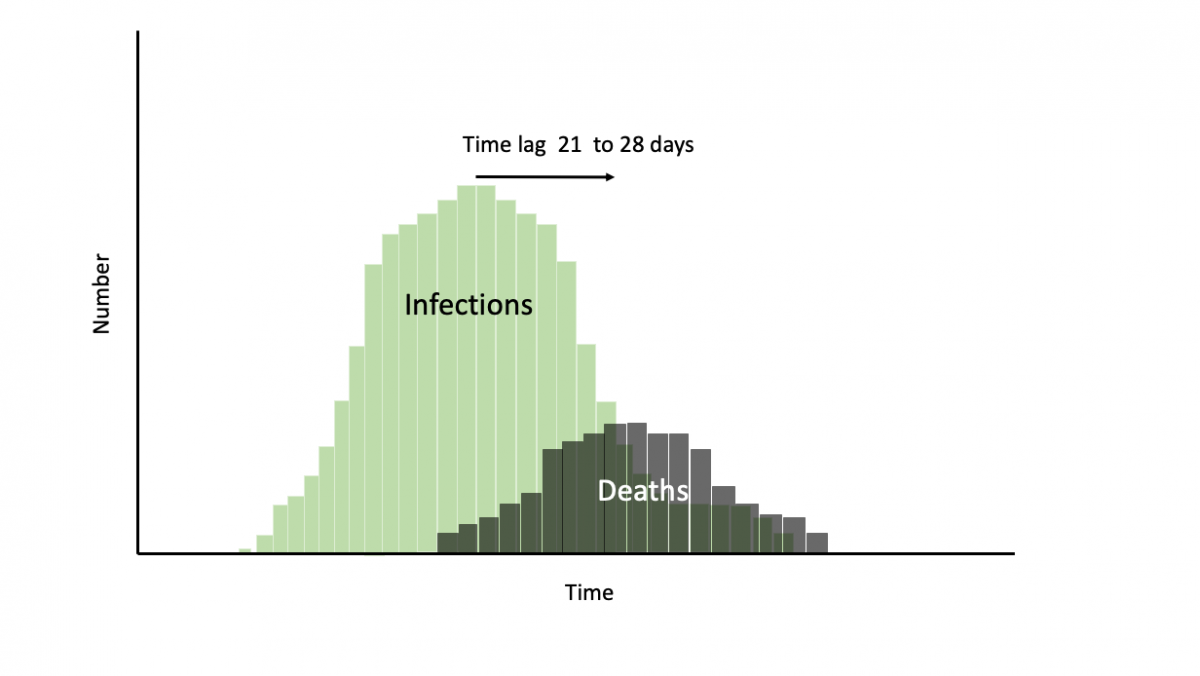
\includegraphics[scale=0.18]{Figures/ss.png}}
\caption{Gaussian-like Approach of Modeling COVID-19}
\label{m3}
\end{figure}


However, when compared to the actual shapes of Italy, a smooth curve is not seen.  It seems to more plateau rather than sharply decline as fast as it rose as shown in Figure \ref{m4}.

 
 \begin{figure}[H]
\centerline{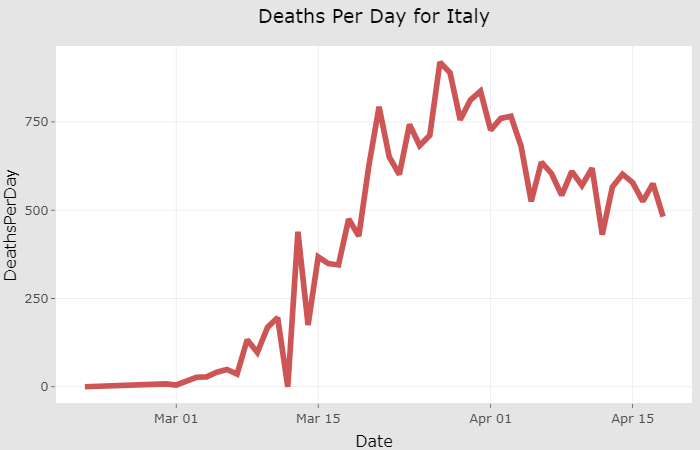
\includegraphics[scale=0.30]{Figures/newplot.png}}
\caption{Italy COVID Deaths Per Day}
\label{m4}
\end{figure}


For Italy and Spain, IHME estimates are passing outside their confidence bounds over the past iterations.  Predictive models that fail to predict two days out within a 95 percent confidence interval are not adequate to model such an important problem. Another caveat of this model is that it is fitted using data from Wuhan which sharply and questionably goes down to 0.  It also fits on data from other countries that are following social distancing and quarantine much more seriously than the United States. Perhaps America's greatest strength is also our greatest weakness when it comes to pandemics, and our quest for freedom and civil liberties are antithetical to containing this disease.
 
 Other models have similar drawbacks.  Notably, the CovidActNow model over-forecasts in the other direction.  It assumes very high R\typesubscript{0} with social distancing, inflating future fatalities and the spread of the disease.  With reported R\typesubscript{0} of under 1 in New York, it is hard to believe their initial assumed 2.1 R\typesubscript{0} is accurate.  Additionally, the CovidActNow model is focused on modeling the disease with assumptions rather than curve fitting.  The Los Alamos National Lab Forecasting team's model has performed the most accurately of all discussed models.  The strengths of the Los Alamos model is that they do not make any assumptions about R\typesubscript{0} except that it will eventually trend downwards. Next they randomly sample all possibilities of the growth rate over time to achieve their forecast.  
 
 \begin{figure}[H]
\centerline{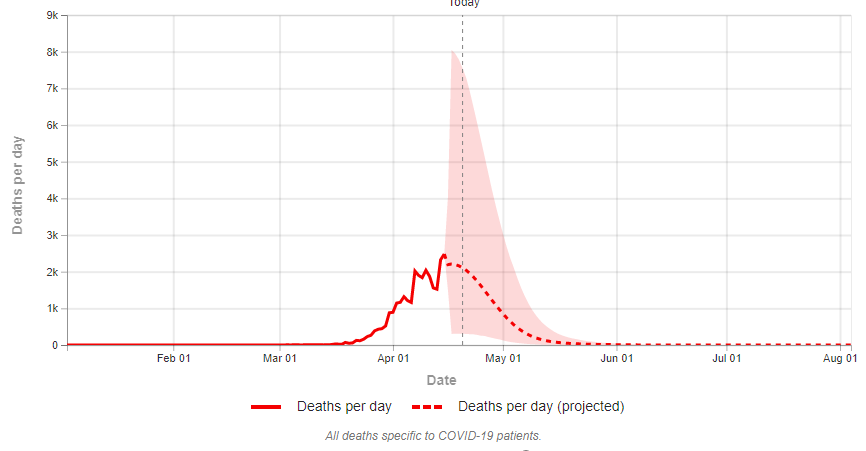
\includegraphics[scale=0.35]{Figures/2.PNG}}
\caption{IMHE Daily Death Model}
\label{m4}
\end{figure}
\section{Conclusions}
\graphicspath{{Figures/}{../Figures/}}


COVID-19 has been a massive challenge for the United States healthcare system.  It is not only causing high mortality, but rippling through the entire economy as companies are shut down, people are out of work, and demand for commodities such as oil are tanking.  It is important to model and forecast the impacts of COVID-19 in order to address the systemic risk in our health systems.  There is no real playbook on what the future looks like with COVID-19, with an incomplete time series and lack of knowledge on a novel virus.

While there are many cited models out there forecasting daily deaths, it is a very tough problem to accurately predict without making many assumptions.  Some models perform better than others, and all face the issue small invalid assumptions spiraling out of control when modeling a virus as infectious as this.   However, having multiple models can help increase understanding of the disease, yielding more useful results for decision-makers. Variables not accounted for include:  under reported deaths, lack of testing to accurately gauge the amount of cases, lack of clarity on immunity periods after infection, and general lack of knowledge on a brand new disease.  It is impossible to know the true hospitalization rate, infection rate, and R\typesubscript{0} without fully knowing the number of undiagnosed cases, which is an almost impossible task in a country with a population of 328 million. Additionally, modeling the disease with symmetric Gaussian-like curves may be not the right approach, as shown in the shapes of daily deaths in Italy and Spain reaching plateaus rather than a sharp decreasing slope.

As the future of this disease unfolds, it will be interesting to see the impacts of social distancing, quarantine, and stay at home orders had on its spread.  Additionally, if everything opens back up and returns to normal, it will be critical to monitor spread in order to limit as few deaths and as much strain as possible on our healthcare system.  The dynamic model developed in this analysis can adapt to different assumptions, and hopefully provide a useful prediction for the United States future.












\bibliographystyle{IEEEtran}
\bibliography{References}

\end{document}
